\documentclass[12pt]{article}
\usepackage{multirow}
\usepackage{graphicx}
\begin{document}
\title{Computer Science M151B, Homework 3}
\date{April 23rd, 2018}
\author{Michael Wu\\UID: 404751542}
\maketitle

\section*{Problem 1}

\paragraph{a)}

\begin{figure}[ht]
    \begin{center}
        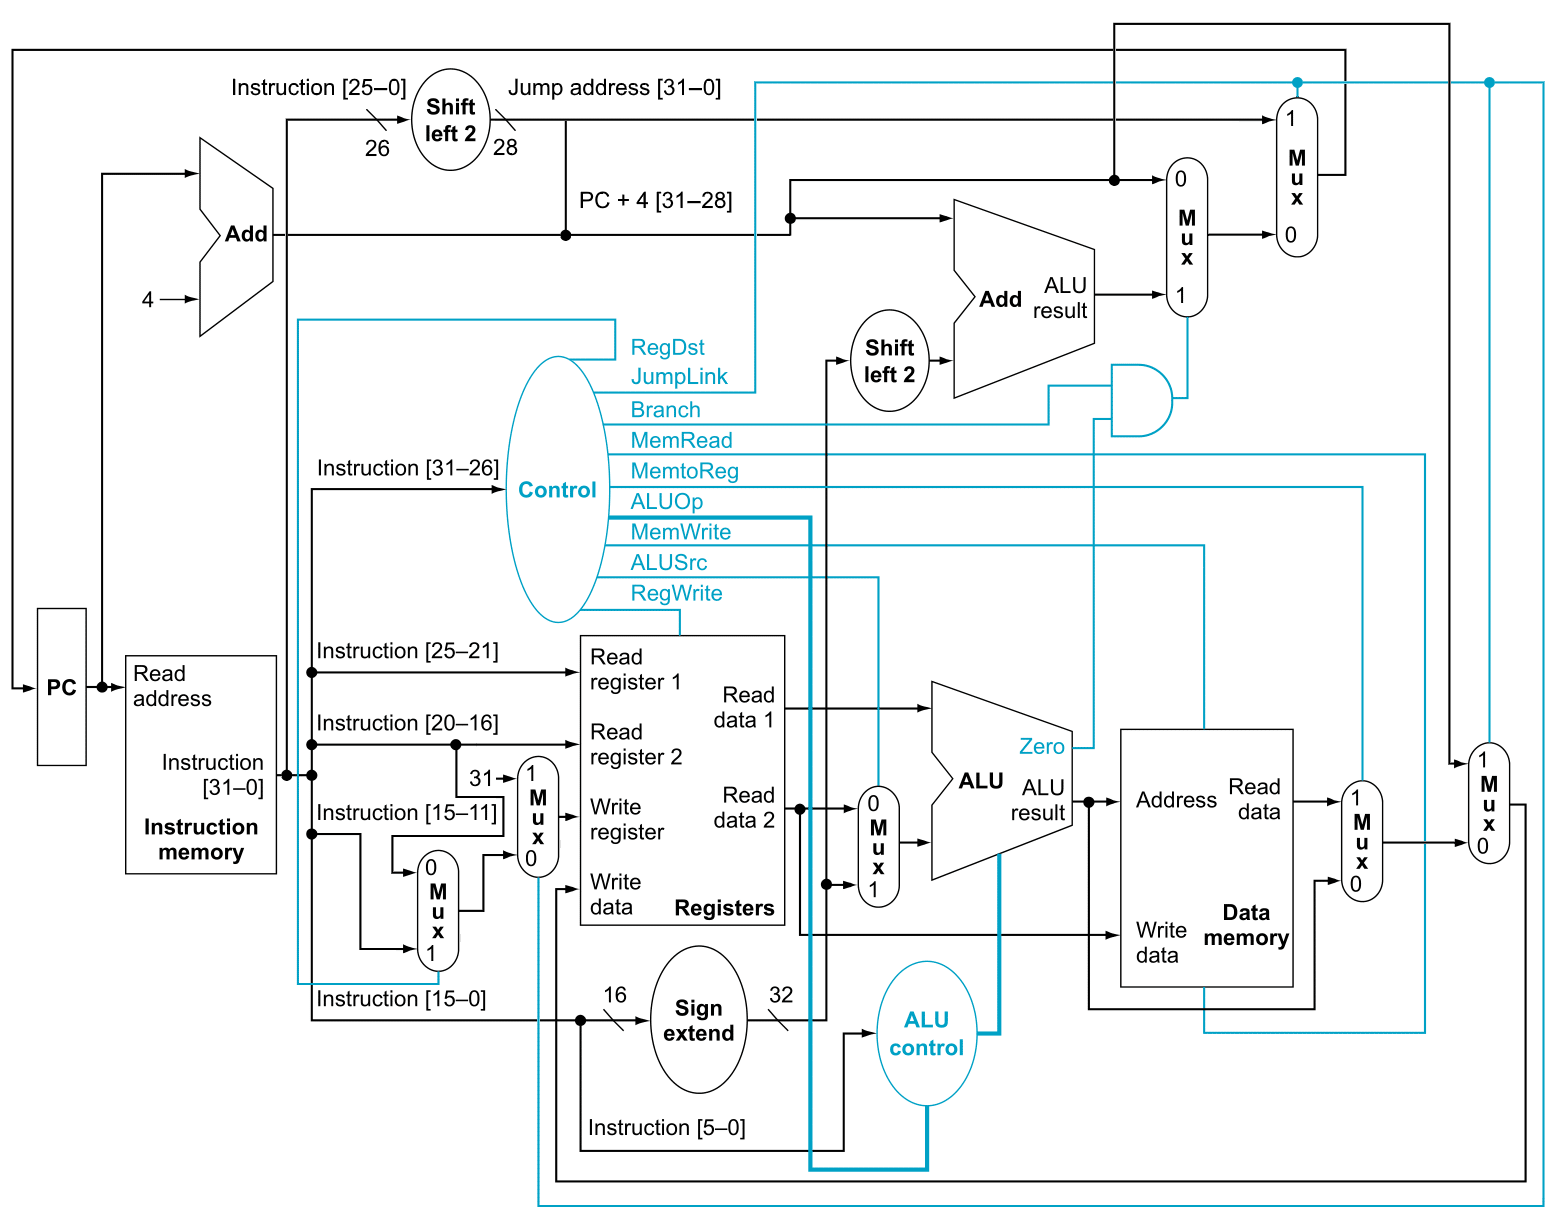
\includegraphics[width=4.4in]{problem1a.png}
    \end{center}
\end{figure}

I have added three multiplexers, one to update the program counter to the target value, one to input the next instruction as a write
value, and one to select register \(31\), which corresponds to \texttt{\$ra}. On the upper left the target value is shifted left by \(2\)
bits and the upper \(4\) bits of the program counter are concatenated on the left of the resulting value, giving a single \(32\) bit address
for the program counter to jump to. A single new control signal \texttt{JumpLink}, controls these multiplexers.

\paragraph{b)}

\texttt{JumpLink} is the new control signal required. This should be \(1\) during the \texttt{jal} instruction, and controls multiplexers that
cause the program counter to jump to the target address and saves the next instruction in register \texttt{\$ra}.

\paragraph{c)}

\begin{center}
        \begin{tabular}{c|c|c|c|c|c|c}
                Input or Output & Signal & R-Format & lw & sw & beq & jal\\
                \hline
                \multirow{6}{*}{Inputs} & Op5 & \(0\) & \(1\) & \(1\) & \(0\) & \(0\)\\
                & Op4 & \(0\) & \(0\) & \(0\) & \(0\) & \(0\)\\
                & Op3 & \(0\) & \(0\) & \(1\) & \(0\) & \(0\)\\
                & Op2 & \(0\) & \(0\) & \(0\) & \(1\) & \(0\)\\
                & Op1 & \(0\) & \(1\) & \(1\) & \(0\) & \(1\)\\
                & Op0 & \(0\) & \(1\) & \(1\) & \(0\) & \(1\)\\
                \hline
                \multirow{10}{*}{Outputs} & RegDst & \(1\) & \(0\) & x & x & x\\
                & ALUSrc & \(0\) & \(1\) & \(1\) & \(0\) & x\\
                & MemtoReg & \(0\) & \(1\) & x & x & x\\
                & RegWrite & \(1\) & \(1\) & \(0\) & \(0\) & \(1\)\\
                & MemRead & \(0\) & \(1\) & \(0\) & \(0\) & \(0\)\\
                & MemWrite & \(0\) & \(0\) & \(1\) & \(0\) & \(0\)\\
                & Branch & \(0\) & \(0\) & \(0\) & \(1\) & \(0\)\\
                & ALUOp1 & \(1\) & \(0\) & \(0\) & \(0\) & x\\
                & ALUOp2 & \(0\) & \(0\) & \(0\) & \(1\) & x\\
                & JumpLink & \(0\) & \(0\) & \(0\) & \(0\) & \(1\)
        \end{tabular}
\end{center}

\section*{Problem 2}

\begin{verbatim}
recf:
  addi $sp, $sp,   -12
  sw   $ra, 0($sp)
  sw   $s0, 4($sp)
  sw   $s1, 8($sp)
  addi $t0, $zero, 1
  beq  $a0, $zero, baseCase0
  beq  $a0, $t0,   baseCase1
  add  $s0, $a0,   $zero
  srl  $a0, $s0,   2
  addi $a0, $a0,   1
  jal  recf
  add  $s1, $v0,   $zero
  srl  $a0, $s0,   1
  addi $a0, $a0,   -1
  jal recf
  add  $v0, $s1,   $v0

finish:
  lw   $ra, 0($sp)
  lw   $s0, 4($sp)
  lw   $s1, 8($sp)
  addi $sp, $sp,   12
  jr   $ra

baseCase0:
  addi $v0, $zero, 3
  ja finish

baseCase1:
  addi $v0, $zero, 2
  ja finish
\end{verbatim}

\section*{Problem 3}

\paragraph{a)}

Yes.

\paragraph{b)}

In a single cycle implementation, the number of cycles that a program takes to execute will be fixed. This is because each instruction takes one cycle,
and the program will run a fixed number of instructions. So the only way that a program can change speed is if the time for a cycle changes. The time
of a cycle is determined by the longest execution path in our implementation. So increasing the length of time of an \texttt{or} operation could increase
the cycle time, if the \texttt{or} operation is on the longest execution path.

\paragraph{c)}

No.

\paragraph{d)}

Within the ALU is a ripple carry adder, which typically takes much more time to finish execution than the \texttt{or} gate. Electrical signals must propagate all
the way through the adder, so this execution path should be much longer than the execution path for the \texttt{or} operation. Thus the \texttt{or} operation
is most likely not on the longest execution path, and doubling its time would not increase the cycle time. Thus it is most likely that the execution time of the
program would not change.

\section*{Problem 4}

\section*{Problem 5}

\paragraph{a)}

\paragraph{b)}

\paragraph{c)}

\paragraph{d)}

\paragraph{e)}

\end{document}